\chapter{接口误用缺陷检测工具集与应用}
\label{cha:tools}
在代码质量保障方法中,规约描述语言能够有效地描述接口使用的约束条件,
高效的检测算法能够对大规模程序进行缺陷检测。
然而,这些已有成果离不开面向实际应用场景工具集的支持。
直观地说,工具决定语言描述、缺陷检测等成果在实际中的应用效果。
本文将第\ref{cha:impsec}章和第\ref{cha:imchecker}章的研究成果应用于实际项目中,
并将结果总结在本章中。
具体来说,本章包含两部分内容:C程序接口误用缺陷数据集APIMU4C和
可视化支持的C程序接口误用缺陷检测工具集Tsmart-IMChecker。
APIMU4C包含对开源项目调研中总结的接口误用缺陷案例库,
以及针对C程序的接口误用测试数据集。
Tsmart-IMChecker工具集包含三个子工具,
以帮助使用者方便高效地撰写IMSpec规约、执行分析引擎并基于差异性对比的方式分析检测结果。
此外,本章将Tsmart-IMChecker工具集应用于实际开源项目中,并对应用结果进行总结。
从全文的研究体系上看,
本章的工作旨在将接口使用约束描述语言IMSpec和规模化检测方法IMChecker应用于实际项目中,
是本文研究工作的应用结果。

\section{引言}
过去的十几年内,研究人员与开发人员面向C程序接口误用缺陷检测投入大量的时间和努力
进行算法设计和工具实现。
例如,微软公司接口缺陷检测项目SLAM,
被广泛使用的开源静态分析工具Cppcheck和Clang Static Analyzer等等。
特别地,为给使用者提供更好的用户体验,这些工具都提供良好的工具接口,
即通过命令行的方式直接调用工具进行检测或者提供可视化支撑的GUI工具。
然而,针对当下的开发环境和程序特点,以上方法存在若干不足。
为弥补现有工作的不足,
本文在第\ref{cha:impsec}章和第\ref{cha:imchecker}章分别提出基于缺陷模式的接口使用约束领域特定语言IMSpec,
以及基于约束描述的规模化接口误用缺陷检测方法IMChecker。
本章将这两部分研究内容进行整理和封装,应用于实际开源项目中,并对应用结果进行总结。

首先,为帮助研究人员和开发者更好地理解接口误用缺陷,
本章将缺陷调研以及算法评估中的原始数据集进行整理和封装,
形成C程序接口误用缺陷数据集APIMU4C(API-misuse for C)。
APIMU4C包含三个模块:
(1)面向Git版本控制库的修改记录挖掘工具Gitgrabber,
(2)开源项目接口误用案例库,
(3)基于公开数据集合以及实际项目案例的接口误用测试数据集。
APIMU4C包含本文中所有的原始数据集,
同时研究人员和开发者可以利用Gitgrabbger对其他领域的缺陷修复进行挖掘和提取。
此外,接口误用测试数据集能够帮助研究人员和开发者对现有工具进行评估,
从而设计更具针对性的检测算法、选择适用的工具进行特定种类的缺陷检测。


为提高工具的实用性减轻使用者的负担,现有工具多提供良好的用户接口。
这些工具面向的领域和对象不同,具有各自的特点。
针对IMSpec语言和IMChecker检测方法,本文设计并开发图形化支撑的工具集Tsmart-IMChecker,
以提供更好的用户体验。
该工具集共包含三个主要模块:
(1)图形化规约撰写工具IMSpec-writer,通过点击、选择和填入必要语义信息的方式,辅助开发者撰写接口使用约束;
(2)静态分析引擎IMChecker,通过对IMChecker方法的实现和封装,
帮助开发者通过命令行的方式直接调用分析引擎并生成对应的缺陷分析报告;
(3)图形化结果展示工具IMDisplayer,通过差异性结果展示的方式帮助使用者快速准确地定位、理解缺陷。

本章将Tsmart-IMChecker应用于实际开源项目中,以评估工具的实用性。
本文将工具集应用于Linux内核、OpenSSL安全库和Ubuntu的应用软件的最新稳定版本中,
共发现超过100个实际缺陷。
本文将缺陷报告进行整理,共提交75个给相应的开发者进行确认。
目前,62个缺陷报告已经被开发者接收,其中32个已经在主分支中修复。
同时,本章对实际应用中遇到的困难、应用发现进行总结,从而帮助研究人员和开发者设计更好的检测工具。



本章其余部分组织结构如下:
\ref{sec:4.2}节对APIMU4C数据集进行介绍,
\ref{sec:4.3}节介绍Tsmart-IMChecker工具总体架构和各子工具,
\ref{sec:4.4}节给出工具集在开源项目上的应用结果,
最后在\ref{sec:4.5}节总结本章工作。

\section{C程序接口误用数据集}
\label{sec:4.2}
近年来,软件缺陷获得研究人员的广泛关注。
特别地,为有效地比较缺陷检测工具的性能,
研究人员设计、整理面向不同领域和不同目标的数据集。
例如,BugBench~\cite{05-bugbench}是针对C程序的缺陷评估集合,
共包含17个开源项目中的缺陷实例,
其中13个与内存、并发和程序特定语义相关。
Defects4J~\cite{14-issta-defects4j}是面向Java程序的缺陷集合,
共包含来自5个开源项目的357个缺陷实例。
在2016年,Amann等整理MUBENCH~\cite{16-msr-mubench}数据集。
该数据集包含89个Java语言实际项目中的接口误用缺陷。
为能够帮助研究人员和开发者更深入地理解接口误用缺陷,
本章对全文的原始数据以及获得方法进行整理、修改和工具实现,形成C程序接口误用缺陷数据集APIMU4C。
该数据集包含三个部分:面向Git版本控制库的修改记录挖掘工具Gitgrabber、
开源项目接口误用案例库、基于公开数据集合以及实际项目案例的接口误用测试数据集。
本节将对每一个部分进行详细介绍。

\paragraph{Gitgrabber}
对实际项目中的缺陷实例进行分析有利于理解缺陷的本质,
从而帮助定义规约描述语言、设计检测算法。
随着软件复杂的度增加和软件规模的提升,现代软件难以独立完成。
同时,随着网络的发展越来越多的开发团队进行远程办公。
在众多的代码维护方式中,Git版本控制软件是最为广泛使用和最受欢迎的方式。
如图\ref{fig:2-3-description}所示,开发者在使用Git版本控制软件时,
对于每一次修改记录都会提供修改的描述报告。
同时,Git会自动计算修改记录中代码的差异并生成差异报告。
因此,本文设计并实现面向Git版本控制软件的修改记录挖掘工具Gitgrabber。
该工具基于Python语言设计,通过自然语言处理的方式对修改记录进行提取。
Gitgrabber以用户提供的配置文件作为输入,以标记挖掘项目的分支、关键词、
时间区间、个数、文件行数等等。
Gitgrabber提供多层挖掘服务,即在第一层挖掘结果的内容中进行二次检索。
例如,通过缺陷修复的关键词进行缺陷修复相关修改记录挖掘,
再基于某种特定类型的关键词挖掘特定领域的缺陷修复。
Gitgrabber使用方便,只需要提供基于结构化的配置文件并通过如下命令执行,
\begin{lstlisting}[language={bash},
basicstyle=\linespread{0.8}\listingsfont,
numbers=none,
xleftmargin=.3\textwidth]
(*@\textcolor{blue}{python}@*) main.py --config config.yml
\end{lstlisting}
挖掘的结果包括:修改记录报告、差异性报告、修改前文件和修改后的文件。
本文中缺陷模式调研的缺陷实例均来自于Gitgrabber的结果。

\paragraph{接口误用案例库}
理解缺陷模式是设计缺陷检测工具的重要基础。
对实际项目中的缺陷实例进行分析,有利于研究人员和开发者更深入地理解缺陷的本质。
因此,本文将第\ref{cha:impsec}章第\ref{sec:2.3}节中分析的接口缺陷实例进行总结,
形成接口误用案例库。
目前该案例库共包含来自6个项目的830个接口误用缺陷实例,
其中Linux内核283个、OpenSSL127个、FFmpeg126个、Curl134个、FreeRDP119个以及Httpd41个。
本文对830个缺陷进行深入分析和核对,确保这些实例与接口误用相关。
同时,针对于每一个缺陷实例,收录缺陷修复报告、差异性报告、修改前错误版本源文件以及
修改后正确版本源文件。
研究人员和开发者可以对这些案例进行研究,从而设计更具有针对性的接口使用约束描述方法和缺陷检测方法。

\paragraph{接口误用测试数据集}
标准化的缺陷测试集合能够有效地评估缺陷检测工具。
然而,目前并没有针对C程序接口误用缺陷的公开测试集合。
因此,本文基于公开数据集以及实际项目中的缺陷实例,构造C程序接口误用缺陷数据集。
该数据集构成如表\ref{tab:4-2-dataset}所示,
包括2172个人工构造的单文件测试用例和100个实际项目用例。
单文件测试用例来源于广泛使用的公开测试集Juliet Test Suite和ITC~\cite{itc}。
每个测试用例在100-200行之间,涵盖不同的C语言的语法结构。
可以用来对检测工具的的语言支持度和检测策略进行分析。
%测试集的另一部分为实际项目缺陷。
实际项目缺陷用例来源于缺陷调研的结果,并注入到项目的最新版本中,
可以用来评估检测工具在实际项目上的分析能力和效果。
这2272个缺陷集合包含缺陷调研中常见的三种常见缺陷模式。
C程序接口误用测试数据集一方面能够帮助研究人员设计更具有针对性的检测算法;
另一方面可以对现有工具进行评估,帮助研究人员分析现有工具不足。
同时使用者可以通过检测结果对工具的能力进行评估,从而选择更适用的工具。

\begin{table}[t]
	\centering
	\begin{minipage}[t]{0.6\linewidth} % 如果想在表格中使用脚注,minipage是个不错的办法
		\caption{C程序接口误用缺陷测试集组成}
		\label{tab:4-2-dataset}
			\begin{tabular}{cccc}
			\hline
			缺陷位置 & 数目& 类型& 代码规模\\
			\hline
			单文件 & 2172 & 人工构造 & 100-200\\
			OpenSSL & 50 & 实际缺陷注入 & 454k\\
			Curl & 30 & 实际缺陷注入 & 113k\\
			Httpd & 20 & 实际缺陷注入 & 203k\\
			总计 & 2272 & \multicolumn{2}{c}{包含所有调研中出现的缺陷类型} \\
			\hline
		\end{tabular}
	\end{minipage}
\end{table}
\section{工具集组成}
\label{sec:4.3}
软件可信保障工具集Tsmart (Trustworthy Software System Modelling And Verification Toolkit),
是清华大学软件学院软件系统与工程研究所研发的软件系统建模验证工具集。
TsmartV3~\cite{tsmart}工具集在2019年1月发布第三版,
是具有完全自主知识产权,面向软件代码安全可靠性的多维度保障体系。
TsmartV3具有代码合规性分析、缺陷静态检测、缺陷自动修复、并发性属性分析等功能。
工具集可用于自动化地检测软件系统中难以发现和调试的重要缺陷,并给出相应的修复建议,
从而提高软件系统的可靠性、提高软件开发测试效率、减小因为软件缺陷导致的损失。
Tsmart-IMChecker工具集是TsmartV3的重要组成部分,面向C程序接口误用缺陷设计。
本节将对Tsmart-IMChecker的总体架构、模块组成进行介绍。

\subsection{总体架构}
Tsmart-IMChecker是基于可视化支持的C程序接口误用缺陷检测工具集。
如图\ref{fig:4-3-overview}中所示,
工具集包含三个主要模块:
\begin{enumerate}
	\item IMSpec规约撰写工具:尽管IMSpec语言提供一套轻量级、类似程序语言的结构化语法形式,
	手动撰写规约是一件耗时、容易出错的工作。
	因此本文设计可视化支撑的IMSpec规约撰写工具,
	帮助用户描述接口使用约束。
	\item IMChecker分析引擎:本文将规模化检测方法封装于IMChecker分析引擎中,
	并提供基于命令行的使用接口。用户可以直接调用该接口进行缺陷检测,
	也可以将分析引擎嵌入到实际开发环境中,作为第三方插件使用。
	\item IMDisplayer结果展示工具:TsmartV提供基于网页版的可视化结果展示工具。
	为帮助实际用户更好地理解接口误用缺陷发生原因,本文实现基于差异性的结果展示工具。
	通过在同一个项目中,正确使用实例与缺陷实例的对比,突出接口误用缺陷的原因和上下文差别。
\end{enumerate}

\begin{figure}[t]
	\centering
	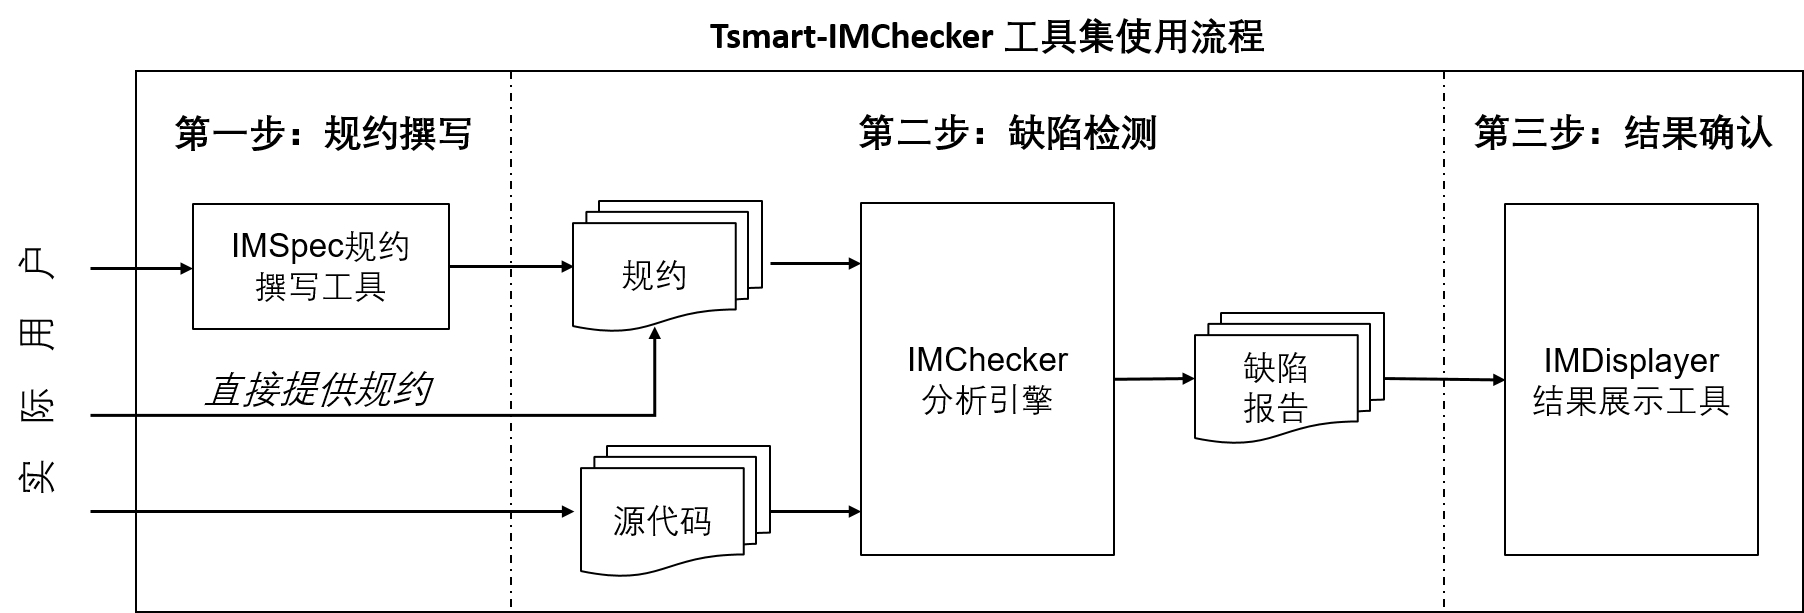
\includegraphics[width=\linewidth]{figures/cp4-overview.png}
	\caption{
		Tsmart-IMChecker工具集使用流程
	}
	\label{fig:4-3-overview}
\end{figure}

用户可以通过三个步骤使用Tsmart-IMChecker工具进行缺陷检测:
撰写规约、缺陷检测和结果确认。
首先,开发者通过IMSpec规约撰写工具,对目标接口的使用约束进行描述。
如果开发者理解IMSpec的语法结构,也可以通过直接撰写文本格式的接口使用约束条件。
在第二步,开发者通过调用缺陷检测引擎,基于提供的约束描述对源代码进行分析。
最后开发者可以直接通过生成的报告核对缺陷检测结果,
也可以通过可视化IMDisplayer工具对检测结果进行确认。
本节将在剩下的内容中对每个模块进行详细介绍。


\subsection{规约撰写模块}
接口使用约束已经被证明能够有效地应用于软件工程领域的不同任务中。
特别地,这些约束能够帮助开发者理解如何正确使用API,
以及帮助测试人员对接口误用缺陷进行检测。
然而人工撰写这些约束条件需要大量的时间与精力,
同时容易在撰写中产生错误。
为减轻使用者撰写IMSpec约束的负担、提高撰写规约语法的准确性,
本文设计并实现图形化支撑的IMSpec规约撰写工具。

如图\ref{fig:4-3-IMSpec-writer}中所示,IMSpec规约撰写工具包含三个部分:
\begin{itemize}
	\item {\kaishu 规约列表}
	界面的最左侧是规约列表,用于展示使用者已经完成的IMSpec接口约束实例。
	用户可以在列表中直观地了解已经完成的约束描述。
	目前,IMSpec撰写工具将一个复杂规约分解成多个子约束,供缺陷分析引擎使用从而提高检测精度。
	因此,显示结果为分解后的约束条件。
	\item {\kaishu 编辑区} 
	界面的右侧为规约编辑区,用于对IMSpec规约进行编辑。
	编辑区包括三大主要区域:目标对象区域、前置条件编写和后置条件编写区域。
	用户在确定目标接口的名称和参数以后,可以在下列的Ref区域选择性地填写与目标API相关的因果调用关系函数。
	例如:目标接口是\texttt{fopen()}函数,
	那么用户可以在Ref区域通过填写\texttt{fclose()}函数地定义进而强化因果调用关系。
	用户可以根据具体的接口使用约束,对前置条件和后置条件进行编辑。
	特别地,IMSpec规约撰写工具在IMSpec语法基础之上,
	在界面显示中进行细微的调整,以提供更直观、准确的功能。
	在规约撰写中,用户可以使用宏定义以保持程序语义一致性和简洁性。
	在缺陷检测阶段提供宏定义的头文件即可。
	\item {\kaishu 文件操作区} 
	界面的左下角是文件操作区域,包括加载宏定义文件、加载文件和导出三个功能。
	
\end{itemize}

\begin{figure}[t]
	\centering
	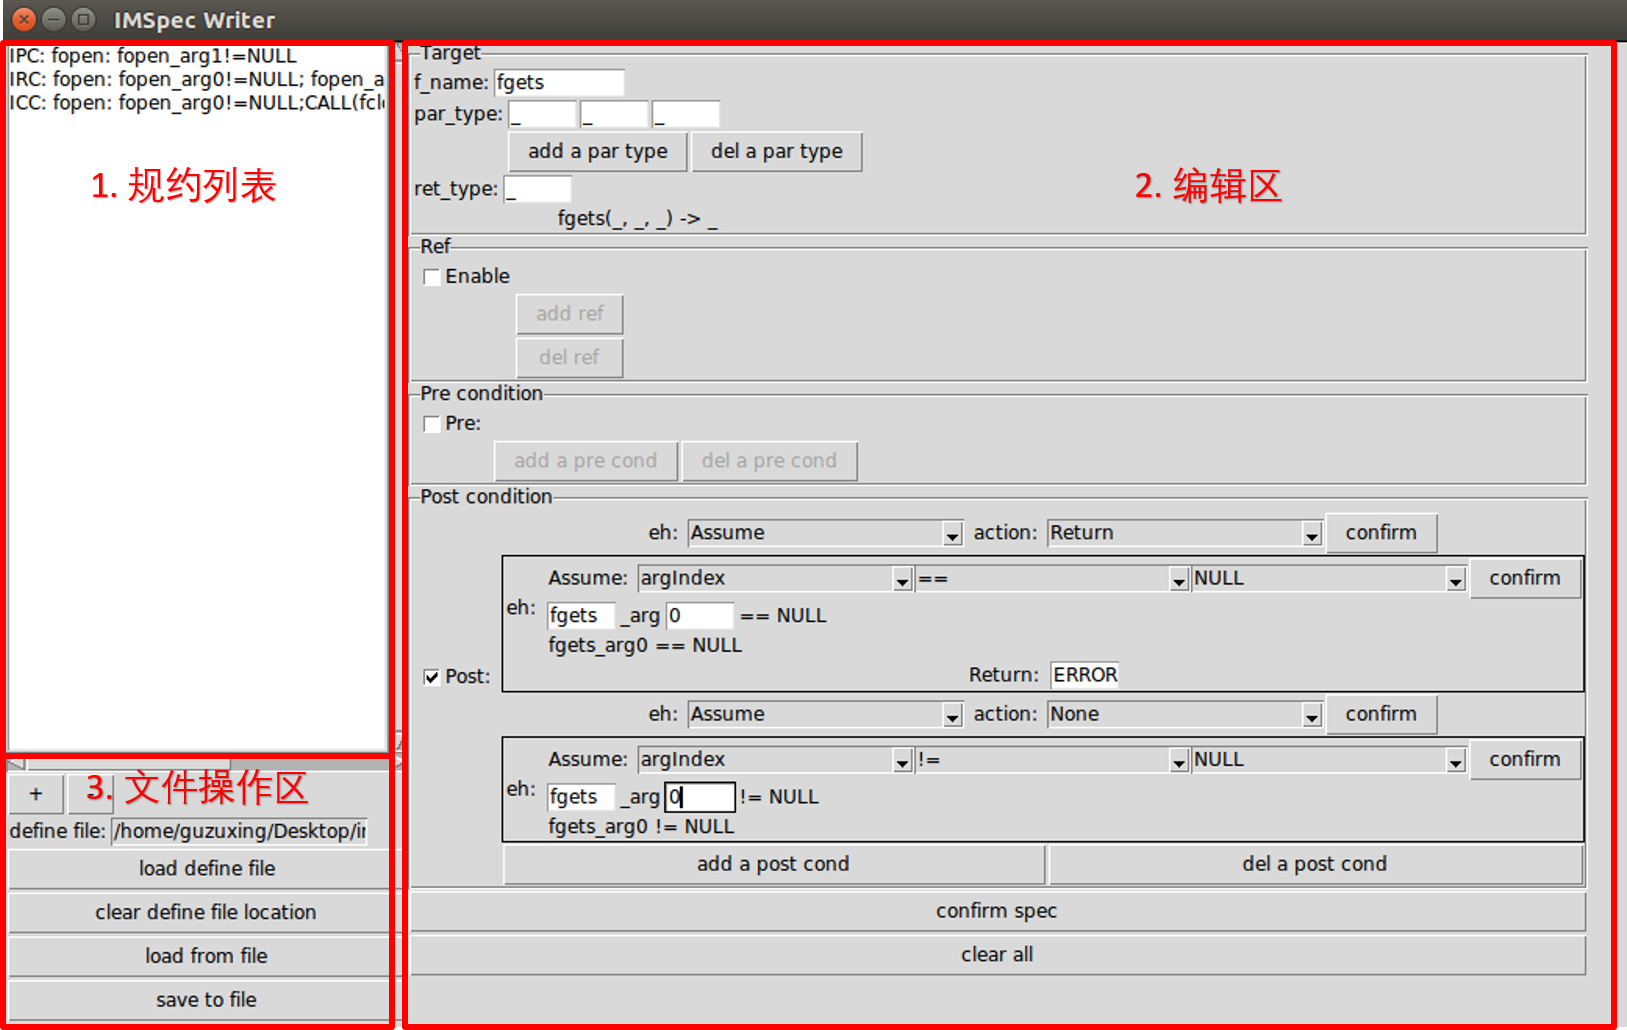
\includegraphics[width=0.85\linewidth]{figures/cp4-IMSpec-writer.png}
	\caption{
		IMSpec规约撰写工具截图
	}
	\label{fig:4-3-IMSpec-writer}
\end{figure}

用户通过命令行,执行imspec\_writer.py文件运行该工具:
\begin{lstlisting}[language={bash},
basicstyle=\linespread{0.8}\listingsfont,
numbers=none,
xleftmargin=.3\textwidth]
(*@\textcolor{blue}{Ubuntu@~:Python3}@*) imspec_writer.py
\end{lstlisting}
其运行结果被保存在用户选择目录的*.yaml文件中,
例如图\ref{fig:2-4-example-imspec}中IMSpec实例。
此外,为帮助使用者维持项目特定的语义及特殊定义,
IMSpec规约撰写工具提供了define.h文件供使用者定义宏参数。
例如,对于图\ref{fig:2-4-example-imspec}中IMSpec实例,
用户可以在define.h中定义如下宏:
\begin{lstlisting}[language={C},
basicstyle=\linespread{0.8}\listingsfont,
numbers=none,
xleftmargin=.3\textwidth]
#define SUCCESS 1
#define FILEERR -1
#define IOERR -2
\end{lstlisting}
在后续解析IMSpec语言时,解析器会进行宏定义的展开从而与程序中的语义保持一致。




\subsection{缺陷检测模块}
\begin{figure}[b]
	\centering
	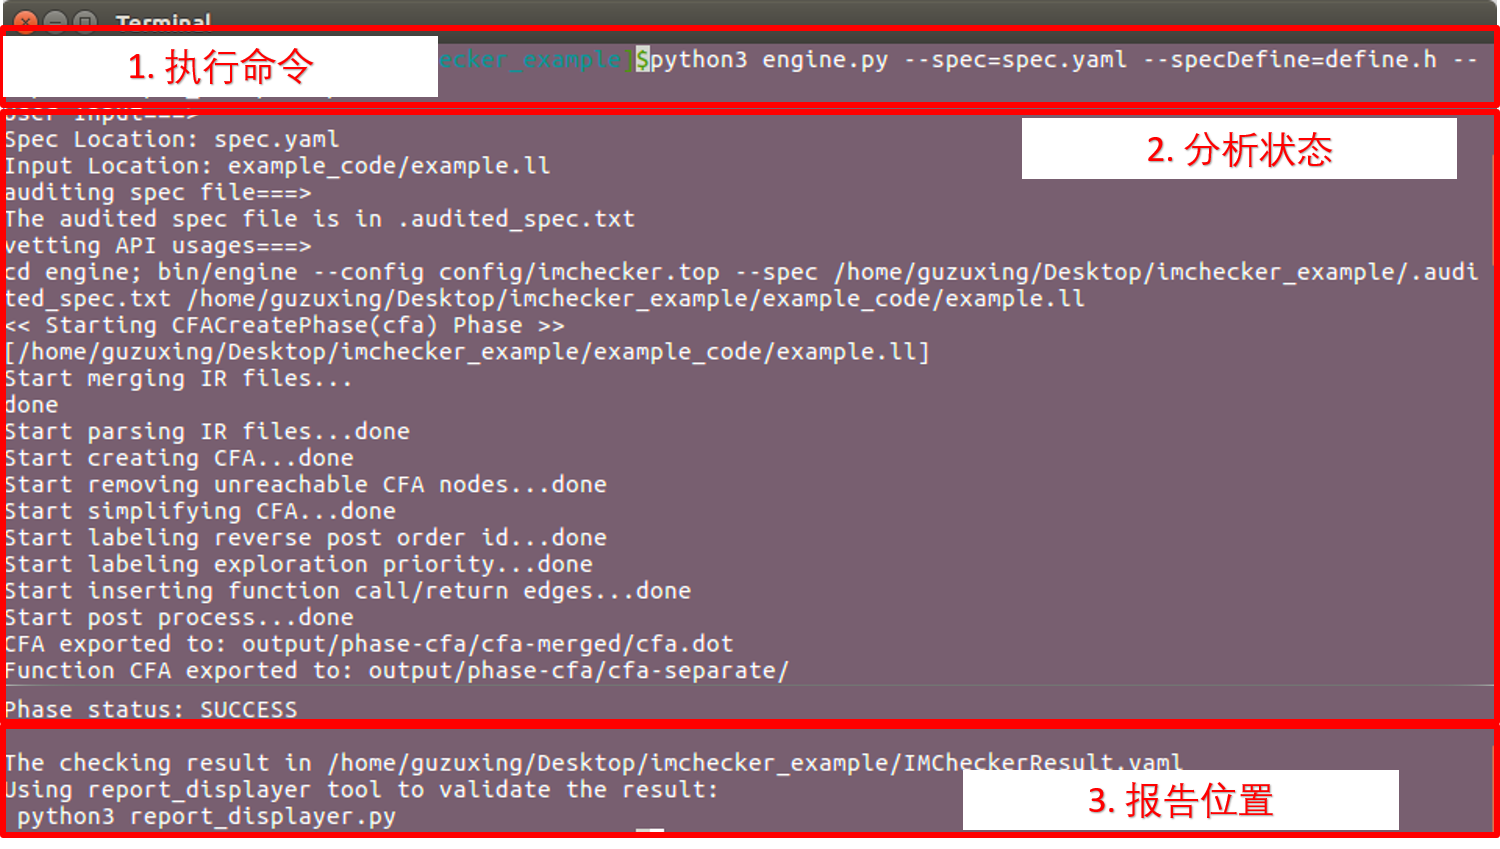
\includegraphics[width=0.85\linewidth]{figures/cp4-IMChecker-engine.png}
	\caption{
		IMChecker分析引擎运行时截图
	}
	\label{fig:4-3-IMChecker-engine}
\end{figure}

研究人员和工具开发人员通过简单易用的用户接口提高工具的实用性,减轻使用者的负担。
特别地,每个工具针对自己应用对象的不同,在工具接口上都有自己的设计目的和特点。
本文对IMChecker方法实现和封装,以命令行的方式帮助开发者直接调用分析引擎,
并生成对应的缺陷分析报告。

如图\ref{fig:4-3-IMChecker-engine}所示,IMChecker分析引擎在命令行中通过直接调用如下指令即可运行,
\begin{lstlisting}[language={bash},
basicstyle=\linespread{0.8}\listingsfont,
numbers=none,
xleftmargin=.1\textwidth]
(*@\textcolor{blue}{Ubuntu@~:Python3}@*) engine.py --spec=XXX --specDefine=XXX --input=XXX
\end{lstlisting}
其中,参数的具体含义如下:
\begin{itemize}
	\item spec: 目标接口使用约束IMSpec文件。
	该文件可以由IMSpec规约撰写工具生成,也可以用户直接根据IMSpec语法进行撰写,
	其内容如图\ref{fig:2-4-example-imspec}中IMSpec实例所示。
	\item specDefine: 规约实例中宏参数的具体定义。在分析阶段,分析引擎会根据宏定义对IMSpec规约进行展开,
	并应用于缺陷检测,
	例如在上文中介绍的define.h文件。
	\item input: 待分析文件。目前,分析引擎在单独使用时
	接受单独可编译的C程序源代码,以及预处理后的LLVM-IR中间表达。
	TsmartV3提供Build-capture编译抓取工具,
	能够自动生成LLVM-IR表达。
	使用者亦可以通过Clang对项目进行编译,通过-S指令生成LLVM-IR表达。
	如果用户通过TsmartV3工具对接口缺陷进行检测,则不需要考虑预处理操作,
	详细使用说明可以参考TsmartV3用户手册~\cite{tsmart}。
\end{itemize}

在分析过程中,IMChecker分析引擎将运行时状态输出到控制台中,以帮助开发者获得分析进展情况。
同时,对于分析中遇到的问题,开发者可以获知原因并进行修复。
如图\ref{fig:4-3-IMChecker-engine}所示,分析引擎首先对IMSpec规约文件进行解析,
接着进入预处理阶段创建CFA、分析阶段,最后针对于分析结果输出到缺陷检测结果报告IMCheckerResult.yaml中。

\begin{figure}[b]
	\centering
	\begin{minipage}{0.7\linewidth}
\begin{lstlisting}[language={C},
basicstyle=\linespread{0.7}\listingsfont,
numbers=none,frame=trBL,
xleftmargin=0pt]
  - (*@\textcolor{blue}{Bug}@*):
    (*@\textcolor{blue}{API}@*): fopen
    (*@\textcolor{blue}{Type}@*): IPC
    (*@\textcolor{blue}{Spec}@*):  fopen==> fopen_arg1!=NULL
    (*@\textcolor{blue}{Reason}@*): Missing or incorrect validation of parameter
    (*@\textcolor{blue}{Error}@*): 
      - IMChecker/tools/example_code/example.c:bad1:14
    (*@\textcolor{blue}{Good}@*): 
      - IMChecker/tools/example_code/example.c:good1:52
\end{lstlisting}
	\end{minipage}
	\caption{
		IMChecker分析结果示例
	}
	\label{fig:4-3-Result}
\end{figure}

IMChecker分析引擎将结果输出到缺陷检测报告中,针对每一个目标API的一种缺陷模式,
缺陷检测结果将汇总在一个“Bug”标签中。
图\ref{fig:4-3-Result}中给出图\ref{fig:2-4-example}中程序检测的一个缺陷实例,其中:
\begin{itemize}
	\item Bug标签为一个目标API某一种缺陷的起始标记符号。
	\item API标签给出目标API的函数名。
	\item Type标签给出缺陷的具体类型。在实际应用场景中,本文将缺陷的类型进行进一步扩展从而展示更具体的缺陷原因。
	例如,IPC表示不正确地参数使用。
	具体参数定义可以参见TsmartV3用户手册。
	\item Spec标签给出导致误用的具体约束条件。图中所描述的约束是第一个参数不可以为NULL。
	\item Reason标签给出基于自然语言的缺陷原因。目前针对于每一个缺陷类型,IMChecker提供一段自然语言描述的缺陷原因。
	\item Error标签给出具体缺陷发生的程序位置。
	\item Good标签给出针对目标API正确使用的程序位置,即满足约束的函数调用位置。
\end{itemize}
如果,该类型的错误存在多个实例或者存在多个正确的使用实例,则Error和Good标签拥有多个实例。
使用者可以通过缺陷检测结果报告对缺陷进行核对,也可以通过IMDisplayer工具进行分析。
此外,该缺陷报告也可以供其他工具的开发者利用。


\subsection{结果展示模块}
\begin{figure}[b]
	\centering
	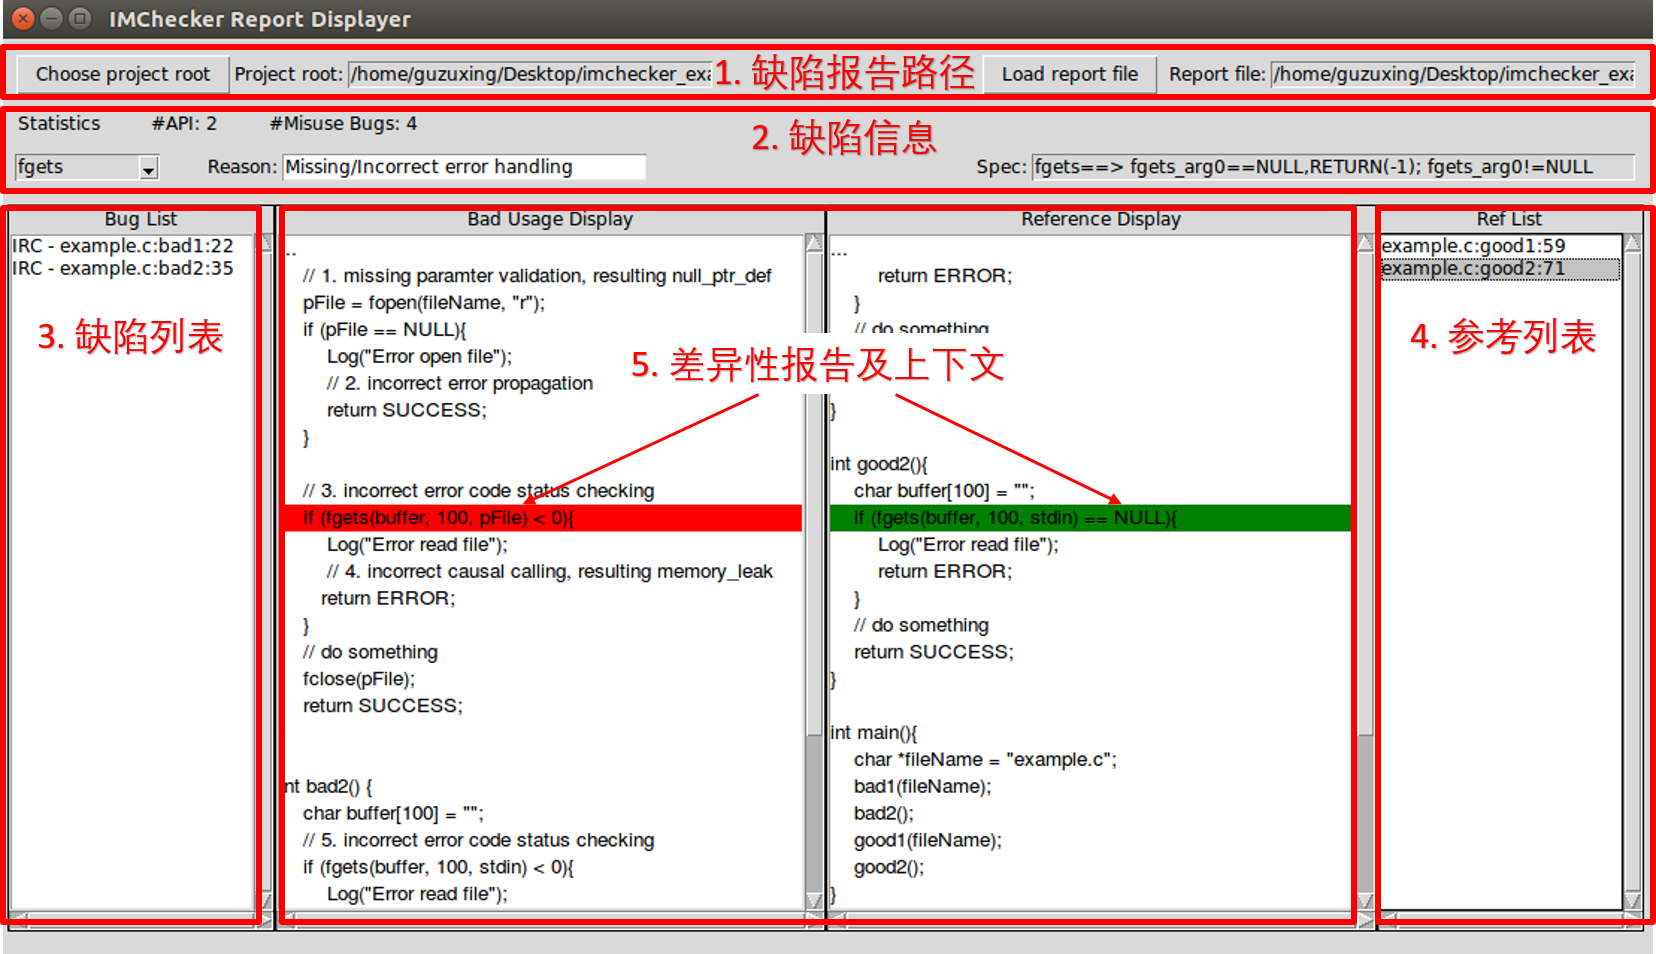
\includegraphics[width=0.85\linewidth]{figures/cp4-IMDisplayer.png}
	\caption{
		IMDisplayer结果展示工具运行时截图
	}
	\label{fig:4-3-IMDisplayer}
\end{figure}

为更好地对缺陷结果进行展示,研究人员和开发者设计并实现各种各样的GUI界面。
针对接口使用和接口误用缺陷的特点,本文设计并实现IMDisplayer结果展示工具,
通过差异性结果对比的方式,帮助开发者深入理解API使用上下文的不同,
并为开发者修复缺陷提供参考。

IMDisplayer结果展示工具在命令行中通过直接调用如下指令即可运行,
\begin{lstlisting}[language={bash},
basicstyle=\linespread{0.8}\listingsfont,
numbers=none,
xleftmargin=.3\textwidth]
(*@\textcolor{blue}{Ubuntu@~:Python3}@*) report_displayer.py
\end{lstlisting}
如图\ref{fig:4-3-IMDisplayer}所示,IMDisplayer工具包含五个部分:
缺陷报告路径选择模块、缺陷信息展示模块、缺陷列表、参考列表以及差异性报告及上下文信息。
用户在使用该工具时,首先要选择缺陷报告的路径信息。
基于缺陷报告,IMDisplayer工具会自动统计缺陷报告中的缺陷实例,
并将误用API数目、缺陷实例数目展示在界面上。
用户通过下拉菜单选择目标API。
如图中所示,目标接口为\texttt{fgets()}函数。
在用户选择目标API后,IMDisplayer工具会更新左侧的缺陷列表,以展示该接口所有误用的情况。
此后,用户可以通过点击左侧的缺陷列表选择具体要审查的缺陷实例。
在用户进行选择后,IMDisplayer会更新缺陷实例的原因、违反的约束,以及右侧参考列表。
用户可以通过对参考列表中的使用实例进行选择,
在缺陷展示框中对缺陷和正确使用进行差异性对比。
例如,图中红色和绿色为缺陷发生的位置和对应的正确使用的位置以及上下文信息。

IMDisplayer的设计动机来源于两点:
(1)IMSpec有效性评估结果显示,相对于自然语言IMSpec规约描述语言对接口使用约束描述更加有效,
即开发者更容易理解使用约束的条件。
因此,作者将缺陷具体违反的约束IMSpec形式展示在界面中,帮助开发者理解缺陷发生的原因。
(2)在应用阶段,开发者提交缺陷报告给对应的开发者。
最初只提供缺陷发生的原因和路径信息,
开发者则表示如果能提供过多的语义信息将有助于理解缺陷的原因。
因此,作者扩展缺陷分析引擎IMChecker,并设计IMDisplayer工具。
特别地,在分析过程中将正确使用的路径进行记录。
在IMDisplayer中,通过差异性比对的方式展现缺陷和正确使用代码片段。
不仅能够有效地帮助使用者理解缺陷的原因,同时能够提供缺陷修复的参考代码。
(3)IMDisplayer独立于分析引擎,通过解析缺陷报告中的标签来展示。
因此,该工具能够扩展到其他应用场景。

\section{案例应用}
\label{sec:4.4}
本文工作旨在对实际项目中C程序接口误用缺陷进行检测,以提高代码质量、应对现代软件开发的迫切需求。
因此,本章将Tsmar-IMChecker工具应用于广泛使用的开源项目中评估本文研究的有效性。
本小结将对应用对象和方法进行介绍、总结应用的结果、
并讨论实际应用中的发现和不足,
为研究人员和开发人员提供思路。

\subsection{实验准备}
\paragraph{应用对象}
本文选取三个典型领域的开源项目作为应用对象,评估Tsmar-IMChecker工具在实际项目中的有效性,
包括:操作系统Linux内核、广泛使用的第三方库OpenSSL安全库和
使用第三方库的应用软件。
其中,应用软件为Ubuntu16.04中,使用OpenSSL安全库的应用软件。
Ubuntu系统提供多个版本的OpenSSL安全库的实现,
本文采用libssl1.0.0\footnote{https://packages.ubuntu.com/xenial/libssl1.0.0}作为应用对象。

应用软件的选择步骤如下。
首先,本文通过Ubuntu系统提供的软件包依赖管理工具搜索所有使用libssl1.0.0的应用软件包,
即通过如下命令,
\begin{lstlisting}[language={bash},
basicstyle=\linespread{0.8}\listingsfont,
numbers=none,
xleftmargin=.25\textwidth]
(*@\textcolor{blue}{Ubuntu@~:}@*) apt-cache rdepends libssl1.0.0
\end{lstlisting}
\texttt{apt-cache rdepends}命令\footnote{http://manpages.ubuntu.com/manpages/bionic/man1/apt-rdepends.1.html}
能够查看一个软件包被哪些软件包所依赖。
搜索的结果显示,超过1200应用软件包依赖于libssl1.0.0。
接着,对于这些软件包本文在Github中搜索是否存在这些软件包的源代码。
目的在于找到这些应用对象中哪些仍然活跃于开源社区中,
从而提交的缺陷报告可以及时获得回复。
对于软件包进行编译、分析需要大量的时间,
因此本文共选择15个广泛使用、不同应用领域、开发者持续维护的应用软件。
为有效评估Tsmar-IMChecker的检测能力(是否能够发现未知的接口误用缺陷),所有应用对象选择截止至2018年7月10-15日的最新稳定版本,
即Linux内核4.18-rc4,OpenSSL-1.1.1-pre8,以及Ubuntu操作系统中应用软件:
\begin{itemize}
	\item dma: 邮件服务,主分支,86个关注(Star数目)
	\item exim: 邮件服务,版本4.91,393个关注
	\item hexchat: 网络实时聊天,版本2.14.1,1949个关注
	\item httping: 针对HTTP请求的Ping服务,主分支,302个关注
	\item ipmitool: 针对智能平台管理接口(Intelligent Platform Management Interface,IPMI)的控制系统,主分支,122个关注
	\item open-vm-tools: WMware软件管理,版本10.3.0,956个关注
	\item irssi: 通信软件,版本1.1.1,1918个关注
	\item keepalive: 负载均衡管理软件,版本2.0.5,1717个关注
	\item thc-ipv6: IPV6攻击测试软件,主分支,442个关注
	\item freeradius-server: 多协议服务器,主分支,943个关注
	\item trafficserver: 网络代理服务器,版本7.1.3,907个关注
	\item tinc: VPN后台服务,版本1.1-pre16,854个关注
	\item sslplit: SSL/TLS攻击测试工具,主分支,1106个关注
	\item rdesktop: 远程桌面服务,主分支,577个关注
	\item proxytunnel: 网络代理服务,主分支,155个关注
\end{itemize}

\paragraph{目标API}
目标API包括两个部分:
(1)对于Linux内核和OpenSSL,本文将第\ref{sec:2.5}节中撰写的IMSpec约束作为目标API,
旨在通过这些被误用过的API再次对这些项目进行检测,从而观察是否依旧存在误用情况。
(2)对于15个Ubuntu中的应用软件,
本文首先通过GNU cflow\footnote{http://www.gnu.org/software/cflow/}抽取这些应用软件的函数调用图。
基于函数调用图和OpenSSL提供的用户手册,选择调用图中使用OpenSSL库中的接口。
例如在dma项目中,通过cflow和OpenSSL用户手册比对的结果,
本文发现该项目使用OpenSSL中包含\texttt{SSL\_connect()}等17个不同的API。
接着在15个项目中,本文将API的使用情况进行总结,选取至少使用过三次的接口。
最终共选择78个不同的API作为检测目标。
本文将这些目标API的IMSpec规约描述文件公开\footnote{https://github.com/tomgu1991/IMChecker/tree/master/imspec},
供研究人员和开发者使用。

\begin{table}[b]
	\centering
	\begin{minipage}[t]{0.7\linewidth} % 如果想在表格中使用脚注,minipage是个不错的办法
		\caption{Tsmart-IMChecker实际项目应用结果}
		\label{tab:4-4-result}
		\begin{tabular}{cccc}
			\hline
			项目名称 & 缺陷报告总数 & 确认未修复 & 已经修复 \\
			\hline
			Linux内核 & 30 & 20 & 5 \\
			 OpenSSL & 17 & 5 & 12\\
			  dma  & 1 & 0 & 1\\
			   exim   &2  & 0 & 2\\
			    hexchat    & 2 & 1 & 0\\
			   httping & 1 & 1 & 0\\
			   ipmitool  & 1 & 1 & 0\\
			    open-vm-tools   &2  & 0 & 2\\
			     irssi    & 2 & 1 & 0\\
			 keepalive & 2 & 0 & 2\\
			 thc-ipv6 & 2 & 0 & 2\\
			 freeradius-server & 2 & 0 & 2\\
			 trafficserver & 3 & 0 & 0\\  
			  tinc  & 2 & 0 & 2\\
			   sslplit   & 2 & 0 & 2\\
			   rdesktop     & 2 & 0 & 0\\
			      proxytunnel    & 2 & 0 & 0\\
			      总计 & 75 & 29 & 32 \\
			\hline
		\end{tabular}
	\end{minipage}
\end{table}


\paragraph{实验环境}
本文在一台装有64位Ubuntu 16.04的台式机上进行实验。
该机器配有Intel(R) Core(R) i5-3470@3.20GHz-4核心CPU和32GB内存。
Tsmart-IMChecker工具需要通过Clang对项目进行预处理,抽取LLVM-IR的中间表达。
然而,部分项目无法完全被Clang支持,例如Linux内核。
同时,部分项目依赖于旧版本的编译环境或者其他编译库难以满足。
针对于这些情况,本文通过人工编译的方式,对这项目中使用目标API的文件进行单独编译,
并将这些能够编译的文件作为分析目标提供给分析引擎。
为控制分析的时间和输出结果,本文每次分析执行一个目标API。
所有的分析中,本文以3小时作为时间界限,即如果三小时无法完成,则将已有分析结果输出。
对于所有找到的实际缺陷,本文进行缺陷理解和归纳,
并在对应的项目中提交缺陷报告或者提交修改申请(Pull Request)。

\subsection{缺陷检测结果}
%https://github.com/tomgu1991/IMChecker/blob/master/evaluation_data/new_bugs/bug_list.md

如表\ref{tab:4-4-result}所示,
Tsmart-IMChecker工具针对于上述17个开源项目共检测到超过100个实际缺陷,
并对其中75个缺陷进行整理提交缺陷报告。
在第一列中,给出项目的名称;
在第二列中,对缺陷提交总数进行展示;
第三列和第四列分别给出在提交的缺陷中,开发者已经确认但没有修复的个数,
以及开发者确认并且修复的缺陷报告个数。
在所有提交的实际接口误用缺陷报告中,
Linux内核有30个,25个已经被开发者确认,其中5个已经在最新的代码中进行修复与集成。
OpenSSL共报告17个缺陷,全部被开发者确认,其中12个已经被修复并集成到主分支和发布版本中。
Ubuntu系统中的应用软件分别报告1-3个缺陷,每个项目具体数据如表中所示。
综合来看,提交的75个缺陷报告中,61个已经被开发者确认。
在确认的报告中,32个已经被成功修复。
下文将对Linux内核、OpenSSL和Ubuntu应用软件中的缺陷进行详细讨论。

\begin{table}[!b]
	\centering
	\scriptsize
	\setlength{\tabcolsep}{4.25pt}
	\begin{minipage}[t]{0.97\linewidth} % 如果想在表格中使用脚注,minipage是个不错的办法
		\caption{Linux内核-4.18rc4缺陷检测结果}
		\scriptsize
		\label{tab:4-4-linux}
		\begin{tabular}{ccclcc}
			\hline
			\multirow{2}{*}{编号}& 缺陷 & \multirow{2}{*}{误用API} & \multicolumn{1}{c}{文件位置} & 缺陷 & \multirow{2}{*}{状态\footnote{$\checkmark\checkmark$为已经修复的缺陷,$\checkmark$为确认的缺陷,$P$为未确认的缺陷。}} \\
			& 编号 & & \multicolumn{1}{c}{文件名:调用函数} & 种类 & \\
			\hline
1 & 200489 & kzalloc & tlb\_uv.c: \textbf{init\_per\_cpu} & ICC & \checkmark \\
2 & 200505 & alloc\_disk & pktcdvd.c: \textbf{pkt\_setup\_dev}& IEH & \checkmark\checkmark \\
3 & 200511& kzalloc & clk-pxa.c: \textbf{clk\_pxa\_cken\_init} & ICC & \checkmark \\
4 & 200519& devm\_clk\_get & hci\_bcm.c: \textbf{bcm\_get\_resources} & IPU & \checkmark \\
5 & 200521& kzalloc & ip22-gio.c: \textbf{ip22\_check\_gio} & ICC & \checkmark \\
6 & 200533& nla\_nest\_start & ncsi-netlink.c: \textbf{ncsi*\_nl}& IPU & \checkmark\checkmark \\
7 & 200535 & nla\_nest\_start & conntrack.c: \textbf{ovs*\_get}& IPU & \checkmark\checkmark \\
8 & 200537 & nla\_nest\_start & datapath.c: \textbf{queue*\_packet} & IPU & \checkmark \\
9 & 200539 & alloc\_skb & chtls\_cm.c: \textbf{chtls*\_conn} & ICC & \checkmark \\
10 & 200541 & \_\_send*alloc\_skb & team.c: \textbf{team\_*\_get} & ICC & \checkmark \\
11 & 200543 & devm\_kzalloc & gpio-tegra.c: \textbf{tegra\_gpio\_probe}& IEH & \checkmark \\
12 & 200545 & devm\_kzalloc & core.c: \textbf{rsnd\_probe}& IEH & \checkmark \\
13 & 200547 & devm\_kzalloc & atmel*\_output.c: \textbf{atmel\_*\_endpoint} & ICC & $P$ \\
14 & 200549 & pci*ext\_capability & nic\_main.c: \textbf{pci*\_capability} & IPU & \checkmark \\
15 & 200551 & pci*ext\_capability & dpc.c: \textbf{dpc\_probe} & IPU & \checkmark\checkmark \\
16 & 200555 & devm*init\_i2c & hmc5843\_i2c.c: \textbf{hmc5843*\_probe} & IPU & \checkmark \\
17 & 200557 & devm\_ioremap & pata\_pxa.c: \textbf{pxa\_ata\_probe} & IEH & \checkmark \\
18 & 200559 & alloc\_workqueue & fm10k\_main.c: \textbf{fm10k*\_module} & ICC & \checkmark \\
19 & 200561 & ida\_pre\_get & namespace.c: \textbf{mnt*\_id} & IPU & \checkmark\checkmark \\
20 & 200563 & wm831x*\_read & clk-wm831x.c: \textbf{wm831x*prepared} & IEH & \checkmark \\
21 & 200565 & dma\_mapping\_error & qib\_sdma.c: \textbf{qib*send} & IEH & \checkmark \\
22 & 200567 & get\_zeroed\_page & sysinfo.c: \textbf{sysinfo\_show} & IEH & \checkmark \\
23 & 200569 & kzalloc & mach-mx27ads.c: \textbf{mx27ads*\_init} & ICC & $P$ \\
24 & 200571 & kzalloc & board-v7.c: \textbf{i2c\_quirk} & ICC & \checkmark \\
25 & 200573 & kzalloc & coherency.c: \textbf{armada\_*\_init} & ICC & \checkmark \\
26 & 200575 & kzalloc & octeon-irq.c: \textbf{octeon*\_map} & ICC & \checkmark \\
27 & 200577 & kzalloc & gptu.c: \textbf{clkdev*\_gptu} & ICC & $P$ \\
28 & 200579& kzalloc & octeon-irq.c: \textbf{octeon*\_map} & ICC & $P$ \\
29 & 200581 & kzalloc & sysctrl.c: \textbf{clkdev\_add\_pci} & ICC  & $P$ \\
30 & 200583 & kzalloc & msi-xlp.c: \textbf{xlp*\_irqs} & ICC & \checkmark \\
			\hline
		\end{tabular}
	\end{minipage}
\end{table}

\paragraph{Linux内核}
如表\ref{tab:4-4-linux}中所示,在Linux内核中
Tsmart-IMChecker工具共提交30个未被报告的接口缺陷。
针对于每一个缺陷报告,本者首先在Linux的缺陷报告系统\footnote{https://bugzilla.kernel.org}中进行查询,
是否已经有相关缺陷报告。
如果没有,则对缺陷报告进行提交。
在提交报告给开发者后,其中25个已经被开发者确认并收到开发者回复的邮件。
至今,5个已经被维护者接受。
其中2个已经集成到Linux最新版当中,3个在进行代码风格修改。

\begin{figure}[b]
	\centering
	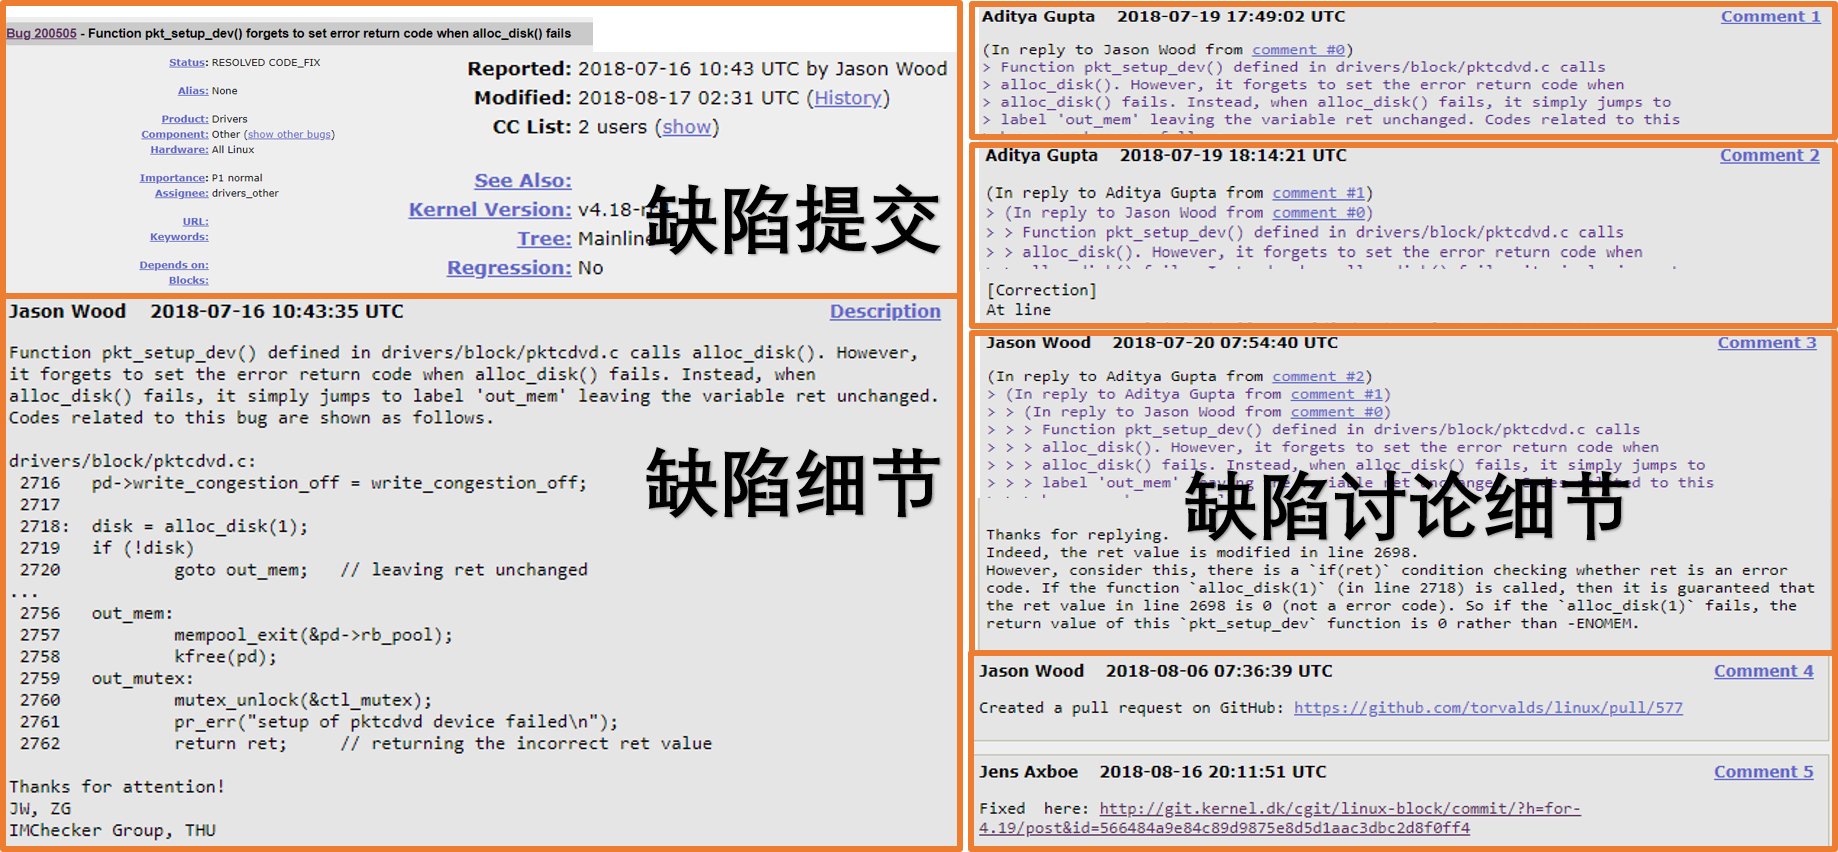
\includegraphics[width=\linewidth]{figures/cp4-linux-example.png}
	\caption{
		Linux接口误用缺陷200505提交和讨论记录
	}
	\label{fig:4-4-linux-example}
\end{figure}

\begin{figure}[t]
	\centering
	\begin{lstlisting}
(*@\textcolor{black}{"summary": "fix setting of 'ret' error return for a few cases",}@*)
"date": "2018-08-16",
"author": "Jens Axboe",
drivers/block/pktcdvd.c
=======================================================
@@ -2740,6 +2740,7 @@ static int pkt_setup_dev(dev_t dev, dev_t* pkt_dev)
pd->write_congestion_on  = write_congestion_on;
pd->write_congestion_off = write_congestion_off;

+	ret = -ENOMEM;
	disk = alloc_disk(1);
	if (!disk)
		goto out_mem;
	\end{lstlisting}
	\caption{
		Linux接口缺陷200505修复细节。
	}
	\label{fig:4-4-linux-example-fix}
\end{figure}


图\ref{fig:4-4-linux-example}为作者将误用接口\texttt{alloc\_disk()}的缺陷实例细节提交以及修复的记录截图。
根据Linux中错误处理机制,接口\texttt{alloc\_disk()}出错时,
外层调用者需要返回\textbf{-ENOMEM}来表示内存不足的错误信息。
然而在drivers/block/pktcdvd.c文件的\texttt{pkt\_setup\_dev()}函数中2718行调用该接口后,
在异常处理路径上并有对返回值进行修改,导致一个不正确的异常处理缺陷(IEH)。
在对该缺陷进行仔细核对后,本文将缺陷提交到Linux缺陷报告系统中,编号为200505。
该缺陷报告在提交后,获得维护者的回复。
在经过三轮的缺陷细节讨论过后,该缺陷被维护者确认,并修改和集成到Linux内核的主分支中。
缺陷修复的细节如图\ref{fig:4-4-linux-example-fix}中所示,
即在返回之前对返回值赋值为错误代码\textbf{-ENOMEM}。


\paragraph{OpenSSL}
\begin{table}[!b]
	\centering
	\scriptsize
	\setlength{\tabcolsep}{4.25pt}
	\begin{minipage}[t]{0.97\linewidth} % 如果想在表格中使用脚注,minipage是个不错的办法
		\caption{OpenSSL-1.1.1-pre8缺陷检测结果}
		\scriptsize
		\label{tab:4-4-openssl}
		\begin{tabular}{ccclcc}
			\hline
			\multirow{2}{*}{编号}& 缺陷 & \multirow{2}{*}{误用API} & \multicolumn{1}{c}{文件位置} & 缺陷 & \multirow{2}{*}{状态\footnote{$\checkmark\checkmark$为已经修复的缺陷,$\checkmark$为确认的缺陷。}} \\
			& 编号 & & \multicolumn{1}{c}{文件名:调用函数} & 种类 & \\
			\hline
1 & 6567 & RAND\_bytes & speed.c: \textbf{RAND*\_loop} & IEH & \checkmark\checkmark \\
2 & 6568 & ASN1\_INTEGER\_get & tasn\_utl.c: \textbf{asn1\_do\_adb} & IPU & \checkmark \\
3 & 6569& ASN1\_INTEGER\_set & p12\_init.c: \textbf{PK*init} & IPU & \checkmark\checkmark \\
4 & 6570& ASN1\_object\_size & asn1\_gen.c: \textbf{generate\_v3 } & IEH & \checkmark \\
5 & 6572& BN\_set\_word & t1\_lib.c: \textbf{ssl*\_dh} & IEH & \checkmark\checkmark \\
6 & 6573& HMAC\_Init\_ex & apps/speed.c: \textbf{HMAC\_loop} & IEH & \checkmark \\
7 & 6574 & EVP\_PKEY\_get0\_DH & statem\_srvr.c: \textbf{tls*\_dhe} & IPU & \checkmark\checkmark \\
8 & 6575 & EC\_KEY\_generate\_key & speed.c: \textbf{run\_benchmark} & IEH & \checkmark \\
9 & 6781 & EC*new*\_name & ec\_ameth.c: \textbf{eckey\_type2param} & ICC & \checkmark\checkmark \\
10 & 6789 & ASN1\_INTEGER\_set & v3\_tlsf.c: \textbf{v2i*FEATURE} & IEH & \checkmark\checkmark \\
11 & 6820 & ASN1\_INTEGER\_to\_BN & ts\_lib.c: \textbf{TS*\_bio} & IPU & \checkmark\checkmark \\
12 & 6822 & BN\_sub & rsa\_ossl.c: \textbf{rsa*\_encrypt} & IEH & \checkmark\checkmark \\
13 & 6973 & EVP\_MD\_CTX\_new & ocsp\_srv.c: \textbf{OCSP*\_sign} & IPU & \checkmark\checkmark \\
14 & 6977 & ASN1\_INTEGER\_set & pk7\_lib.c: \textbf{PKCS7*type} & IEH & \checkmark\checkmark \\
15 & 6982 & OBJ\_nid2obj & asn\_moid.c: \textbf{do\_create} & IEH & \checkmark\checkmark \\
16 & 6983 & BN\_sub & bn\_x931p.c: \textbf{BN*\_Xpq} & IEH & \checkmark\checkmark \\
17 & 7235 & DH\_set0\_key & dh\_lib.c: \textbf{DH*\_key} & IEH & \checkmark \\
			\hline
		\end{tabular}
	\end{minipage}
\end{table}

\begin{figure}[t]
	\centering
	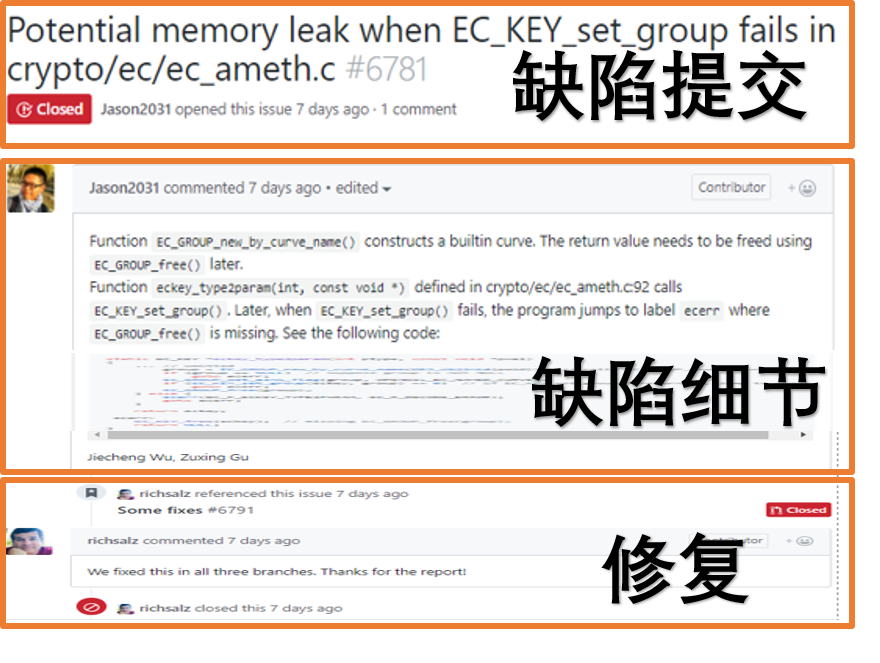
\includegraphics[width=0.8\linewidth]{figures/cp4-openssl-example.png}
	\caption{
		OpenSSL缺陷6781提交和修复记录
	}
	\label{fig:4-4-openssl-example}
\end{figure}



如表\ref{tab:4-4-openssl}中所示,在OpenSSL中Tsmart-IMChecker工具共提交17个未被报告的接口缺陷。
针对于每一个缺陷报告,本文首先在Github中OpenSSL代码库中提交Issue。
在提交报告给开发者后,所有的缺陷报告都获得开发者的回复。
其中12个已经被维护者修复并集成在主分支内,5个被标记为待评估(Assessed)。
OpenSSL与Linux内核的缺陷报告系统不同通过Github的Issue系统维护,
因此缺陷的提交和修复能够获得及时的反馈。

\begin{figure}[t]
	\centering
	\begin{lstlisting}
(*@\textcolor{black}{"summary": "Avoid memory leak on failure path.Thanks to Jiecheng Wu, Zuxing Gu for the report.",}@*)
"date": "2018-07-26",
"author": "richsalz",
=======================================================
@@ -122,13 +122,12 @@ static TLS_FEATURE *v2i_TLS_FEATURE(const X509V3_EXT_METHOD *method,
+   EC_GROUP *group = NULL;
	[...]
	else if (ptype == V_ASN1_OBJECT) {
		const ASN1_OBJECT *poid = pval;
-		EC_GROUP *group;
		[...]
		group = EC_GROUP_new_by_curve_name(OBJ_obj2nid(poid));
		if (group == NULL)
			goto ecerr;
		EC_GROUP_set_asn1_flag(group, OPENSSL_EC_NAMED_CURVE);
		if (EC_KEY_set_group(eckey, group) == 0)
			goto ecerr;
		EC_GROUP_free(group);
	} else {
	[...]
ecerr:
	EC_KEY_free(eckey);
+	EC_GROUP_free(group);
	return NULL;
	\end{lstlisting}
	\caption{
		OpenSSL缺陷6781修复细节
	}
	\label{fig:4-4-openssl-example-fix}
\end{figure}

图\ref{fig:4-4-openssl-example}是作者在OpenSSL项目检测到的一个内存泄漏缺陷。
OpenSSL设计接口\texttt{EC\_GROUP\_new\_by\_curve\_name()}来创建EC\_GROUP对象。
该对象在生命周期结束后需要通过\texttt{EC\_GROUP\_free()}进行释放。
然而在ec\_ameth.c文件的\texttt{eckey\_type2param()}的函数体内,
在一条异常处理路径上开发者并没有进行释放导致一个内存泄漏错误。
如图\ref{fig:4-4-openssl-example-fix}中所示,
开发者在12行进行内存对象的申请,
然而在16行的if判断错误处理中直接通过goto语句跳转到21行继续执行。
因此这条异常处理路径上,忽视了对于12行申请内存对象\texttt{group}的释放。
在作者提交缺陷报告并说明出错路径后,开发者在12小时内完成修复。
修复细节如图\ref{fig:4-4-openssl-example-fix}所示。

OpenSSL项目设计明确的错误代码机制,并在用户手册中提供基于自然语言的描述。
然而,项目的开发者却忽略大量的异常处理检测。
例如,缺陷6572、6789和6982,均由不正确的异常处理原因导致的软件缺陷。
作者在提交缺陷报告后,开发者均进行相应的修复。




\paragraph{应用程序}

\begin{table}[!t]
	\centering
	\setlength{\tabcolsep}{2.25pt}
	\begin{minipage}[t]{\linewidth} % 如果想在表格中使用脚注,minipage是个不错的办法
		\caption{Ubuntu16.04应用软件缺陷检测结果}
		\label{tab:4-4-apps}
		\begin{tabular}{ccclcc}
			\hline
			 项目 & 缺陷 & \multirow{2}{*}{误用API} & \multicolumn{1}{c}{文件位置} & 缺陷 & \multirow{2}{*}{状态\footnote{$\checkmark\checkmark$为已经修复的缺陷,$\checkmark$为确认的缺陷,$P$为未确认的缺陷。}} \\
			名称 & 编号 & & \multicolumn{1}{c}{文件名:调用函数} & 种类 & \\
			\hline
dma & 59 & SSL\_connect & crypto.c: \textbf{smtp*\_crypto} & IEH & \checkmark\checkmark \\
\cline{1-1}
\multirow{2}{*}{exim} & 2316 & X509\_NAME\_oneline & tls-openssl.c: \textbf{x509*\_names} & IEH & \checkmark\checkmark \\
    & 2317 & SSL\_CTX*\_list & tls-openssl.c: \textbf{tls*\_cb} & IEH & \checkmark\checkmark \\
\cline{1-1}
\multirow{2}{*}{hexchat} & 2244 & BN\_set\_word & dh1080.c: \textbf{dh1080\_init} & IEH & \checkmark \\
    & 2245 & DH\_set0\_key & dh1080.c: \textbf{dh1080\_compute\_key} & IEH & $P$ \\
\cline{1-1}
\multirow{1}{*}{httping} & 41 & SSL\_CTX\_new & mssl.c: \textbf{initialize\_ctx} & ICC & \checkmark \\
\cline{1-1}
\multirow{1}{*}{ipmitool} & 37 & MD2\_Init & auth.c: \textbf{ipmi\_auth\_md2} & IEH & \checkmark \\
\cline{1-1}
\multirow{1}{*}{open-} & 291 & SSL\_*list & sslDirect.c: \textbf{SSL\_NewContext} & IEH & \checkmark\checkmark \\
vm-tools & 292 & X509*\_current\_cert & certverify.c: \textbf{VerifyCallback} & IPU & \checkmark\checkmark \\
\cline{1-1}
\multirow{2}{*}{irssi} & 943 & SSL*\_certificate & net*-openssl.c: \textbf{irssi*\_handshake} & IPU & $P$ \\
    & 944 & BIO\_read & certverify.c: \textbf{set*\_info} & IEH & \checkmark \\
\cline{1-1}
\multirow{2}{*}{keepalive} & 1003 & SSL*\_new & ssl.c: \textbf{build*\_ctx} & ICC & \checkmark\checkmark \\
    & 1004 & SSL\_new & ssl.c: \textbf{ssl\_connect} & ICC & \checkmark\checkmark \\
\cline{1-1}
\multirow{2}{*}{thc-ipv6} & 28 & BN\_new & thc-ipv6-lib.c: \textbf{thc\_memstr} & ICC & \checkmark\checkmark \\
    & 29 & BN\_set\_word & thc-ipv6-lib.c: \textbf{thc\_memstr} & IEH & \checkmark\checkmark \\
\cline{1-1}
\multirow{2}{*}{FreeRADIUS} & 2309 & BIO\_new & session.c: \textbf{tls*\_cert} & ICC & \checkmark\checkmark \\
    & 2310 & i2a\_ASN1\_OBJECT & session.c: \textbf{tls*\_cert} & IEH & \checkmark\checkmark \\
\cline{1-1}
\multirow{3}{*}{trafficserver} & 4292 & SSL\_CTX\_new & http\_load.c: \textbf{handle\_connect} & ICC & $P$ \\
    & 4293 & SSL\_new & http\_load.c: \textbf{handle\_connect} & ICC & $P$ \\
    & 4294 & SSL\_write & http\_load.c: \textbf{handle\_connect} & IEH & $P$ \\
\cline{1-1}
\multirow{2}{*}{tinc} & 205 & BN\_hex2bn & tincd.c: \textbf{keygen} & IPU & \checkmark\checkmark \\
    & 206 & RAND\_load\_file & tincd.c: \textbf{main} & IEH & \checkmark\checkmark \\
\cline{1-1}
\multirow{2}{*}{sslsplit} & 224 & SSL*\_certificate & pxyconn.c: \textbf{pxy*\_create} & IEH & \checkmark\checkmark \\
    & 225 & SSL*\_PrivateKey & pxyconn.c: \textbf{pxy*\_create} & IEH & \checkmark\checkmark \\
\cline{1-1}
\multirow{2}{*}{rdesktop} & 280 & BN\_bin2bn& ssl.c: \textbf{rdssl*\_encrypt} & IEH & $P$ \\
    & 281 & BN\_mod\_exp & ssl.c: \textbf{rdssl*\_encrypt} & IEH & $P$ \\
\cline{1-1}
\multirow{2}{*}{proxytunnel} & 36 & SSL\_connect & ptstream.c: \textbf{stream*\_ssl} & IEH & $P$ \\
    & 37 & SSL\_new& ptstream.c: \textbf{stream*\_ssl} & ICC & $P$ \\
			\hline
		\end{tabular}
	\end{minipage}
\end{table}

OpenSSL软件库是网络通信领域广泛使用的安全库,这些接口误用会极大地损害系统的可靠性。
因此,对OpenSSL项目中接口缺陷检测本身具有重要意义。
一方面,可以提高软件库本身的质量;
另一方面,通过完善软件库代码的质量,能够有效地为使用者提供可靠的使用样例。

我们在Ubuntu16.04的应用软件中,对OpenSSL软件库接口缺陷进行检查。
检测结果显式,这些应用软件存在大量的接口误用缺陷。
本文在对结果分析、核对和整理后,
将28检测结果提交到对应的15个项目中。
如表\ref{tab:4-4-apps}所示,28个缺陷中19个被开发者接受,其中15个已经被成功修复。
特别地,dma、exim、open-vm-tools、keepalive、thc-ipv6、FreeRADIUS、tinc和sslplit八个项目,对缺陷报告进行及时的确认和修复。
虽然其他项目对缺陷报告没有修复,但部分报告已经被开发者确认并标记为下一个版本需要处理的问题。
其他报告则处于没有回复的阶段,即开发者并没有否定检测结果为误报。
同时,相应的缺陷模式已经在其他的项目中获得认可。
因此,本文认为这些缺陷具有极高的可信度。

\begin{figure}[t]
	\centering
	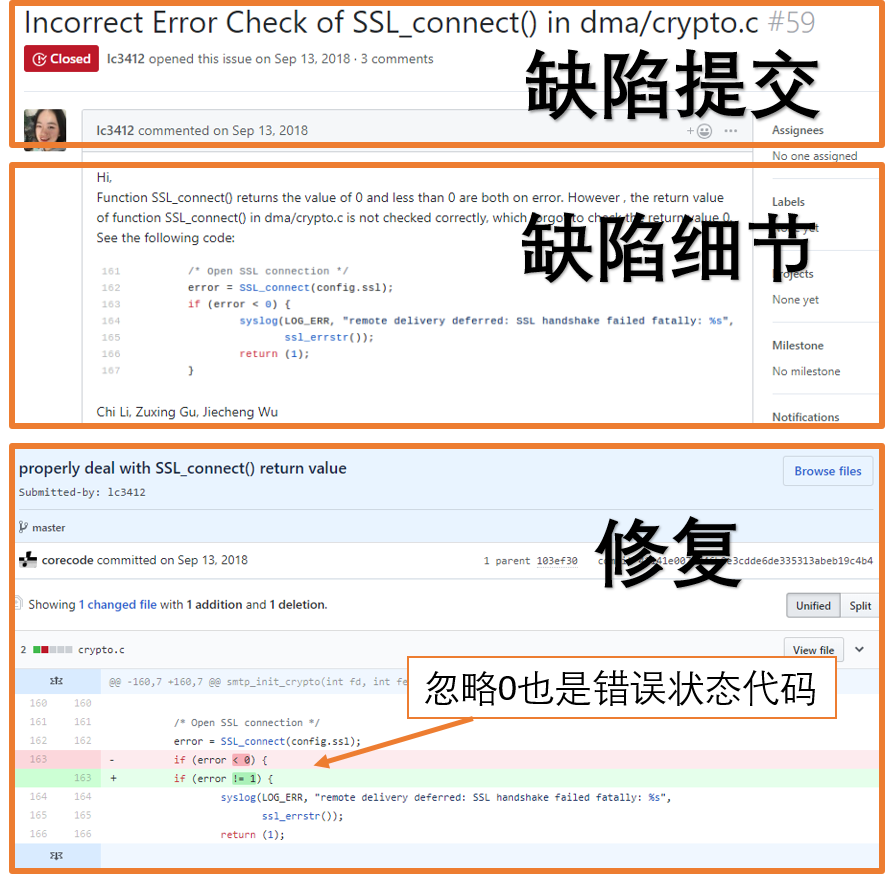
\includegraphics[width=0.8\linewidth]{figures/cp4-dma-example.png}
	\caption{
		dma缺陷59提交和修复记录
	}
	\label{fig:4-4-dma-example}
\end{figure}

图\ref{fig:4-4-dma-example}是本文在dma项目检测到的一个不正确的异常处理错误。
OpenSSL的官方用户手册中指出,接口\texttt{SSL\_connect()}用于初始化TSL/SSL服务器握手操作(handshake)。
根据TSL/SSL协议本身,当握手失败时该函数的实现返回0代表链接被成功关闭,返回负数则代表错误发生在协议层、链接等等。
因此,该接口的错误状态代码有两种情况,针对该函数的异常处理也需要考虑这两种情况。
如图中代码所示,在dma项目中开发者只对负数进行检查,而忽略错误状态代码为0的情况。
因此,当\texttt{SSL\_connect()}函数在执行时返回0时,该项目的异常处理机制将失效,程序的鲁棒性将会被破坏。
dma项目为邮件服务,因此该错误极大可能被攻击者利用从而产生漏洞。
本文在提交缺陷报告后,开发者进行了即使修复。
如图中所示,开发者对错误状态代码的判断进行完善,从而正确执行异常处理机制。



\subsection{应用经验总结}
本文将Tsmart-IMChecker应用于实际开源项目中,
对接口缺陷进行分析并将缺陷报告提交给相应的开发者。
本文将缺陷检测、报告提交、开发者讨论和后续跟进工作中
遇到的困难、发现和项目应用经验总结在下文中。
主要包括如下几个方面:
接口误用缺陷、现有文档、缺陷提交和开发者态度。

\paragraph{接口误用缺陷}
同第\ref{sec:2.3}节调研结果一致,接口误用缺陷并不是个例,普遍存在于各种软件系统中。
特别地,本文共找到超过100个实际缺陷,并提交75个缺陷报告给实际开发者。
其中61个(81.33\%)被开发者接受,32个(42.67\%)已经被开发者修复。
在本文分析之前Linux内核和OpenSSL软件库作为广泛使用的基础软件,
两者代码已经被著名的分析工具(例如,商业工具Coverity~\cite{coverity}和学术工具Clang Static Analysis)检测过。
更严重的是这些缺陷的目标API均从已有的缺陷修改记录中获得,
即这些缺陷已经在过去发生过。
同时,被分析的应用软件中每个都至少误用一个OpenSSL的接口。
%我们在后续的研究中,在其他的应用软件中发现同样的现象。
在对缺陷模式、细节分析后,本文发现这些缺陷产生存在两方面的原因:
(1)软件库开发者间缺少缺陷报告分享机制。
开发者经常会忘记接口使用的约束。
特别地,即使新的代码中存在和过去发生的缺陷的模式一样,
并没有一个能够自动检测的方法,对开发者进行提示。
(2)客户端开发者缺少足够的领域知识,导致误用库函数,
即客户端开发者在使用OpenSSL软件库时,没有深入理解或者参考文档,
导致接口使用错误。

总结来说,开发者在开发过程中难免会产生接口误用,无论是无意忘记约束,还是本身缺少理解。
因此,规模化、高效的分析工具对接口误用缺陷检测具有重要的实际意义。
特别地,Tsmart-IMChecker基于规约描述语言进行检测,
集成大量的领域知识并容易扩展。
同时可以渐进式分析,即可以只应用于新修改的代码中。

\begin{figure}[b]
	\centering
	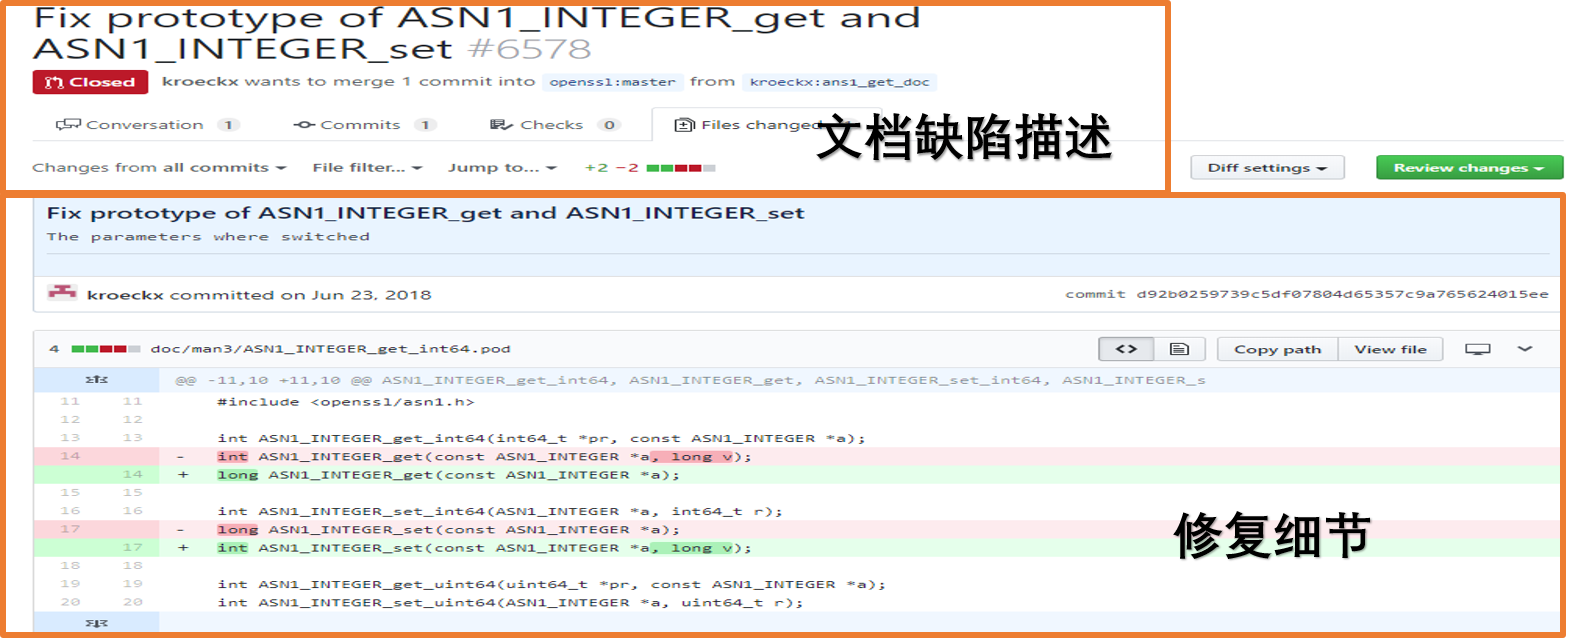
\includegraphics[width=\linewidth]{figures/cp4-doc-bug.png}
	\caption{
		OpenSSL中接口用户手册缺陷修复记录
	}
	\label{fig:4-4-doc-bug}
\end{figure}
\begin{figure}[t]
	\centering
	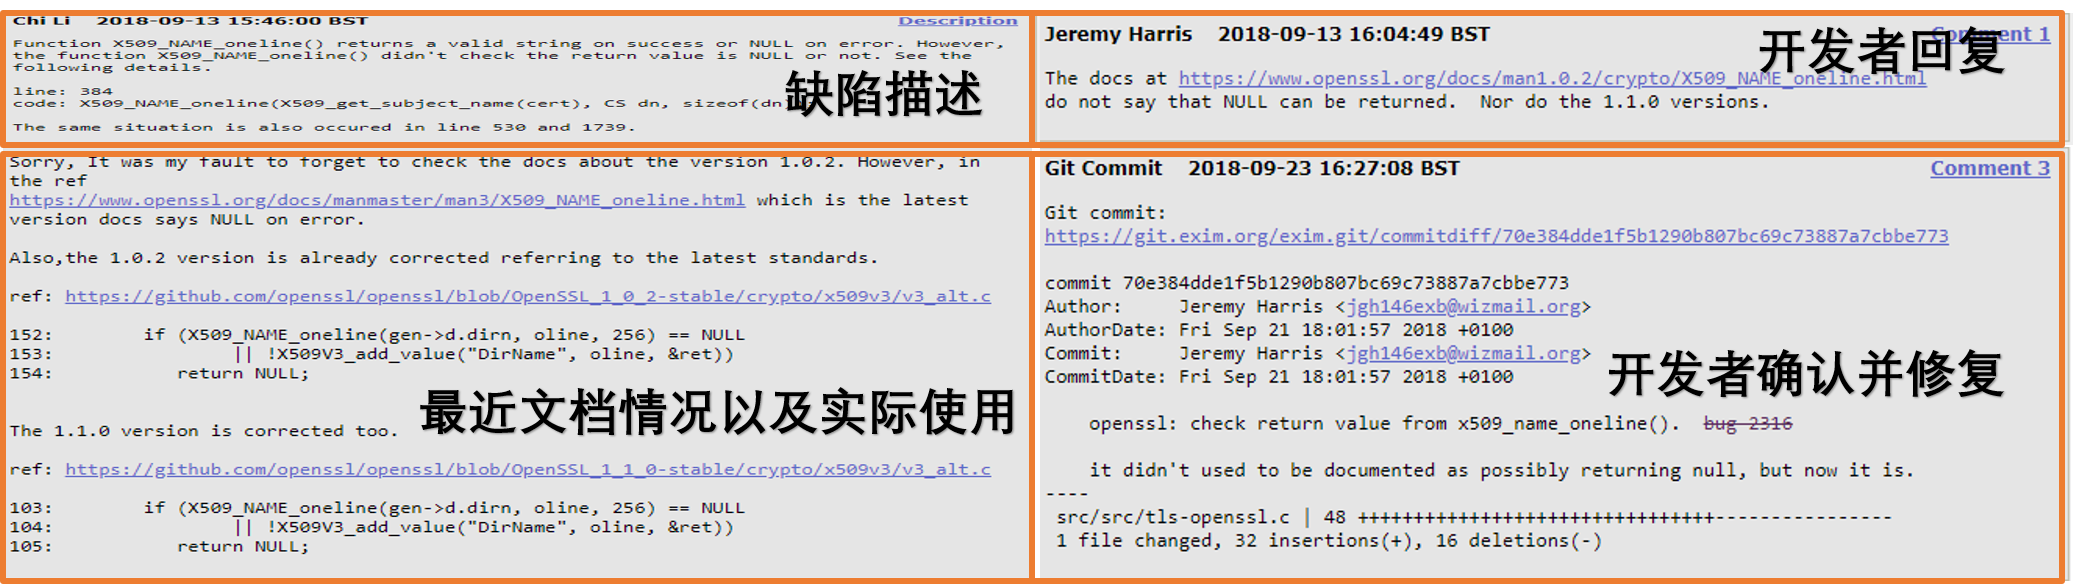
\includegraphics[width=\linewidth]{figures/cp4-exim-bug.png}
	\caption{
		exim项目中缺陷2316修复记录
	}
	\label{fig:4-4-exim-bug}
\end{figure}
\paragraph{现有文档}
虽然OpenSSL软件库为使用者提供格式优良的自然语言描述的接口使用约束和解释,
然而在本文分析的15个应用软件中,依旧存在大量的接口误用缺陷。
对缺陷报告和文档进行分析后,现有的文档存在如下几个不足:
\begin{itemize}
	\item 文档自身存在错误。在OpenSSL的缺陷检测中,本文发现OpenSSL提供的官方文档中存在错误。
	在进行代码具体使用情况和文档描述的核对后,本文提交文档和接口缺陷报告(Issue-6569)。
	开发者在收到缺陷报告后,1天内对文档进行修复,如图\ref{fig:4-4-doc-bug}中所示。
	\item 文档利用率不足。一方面,软件库的代码实现中本身存在对库接口的误用;
	另一方面,客户端开发者对文档参考不足,误用这些接口。
	在和开发者讨论接口误用原因时,超过一半的开发者表示
	在遇到使用问题时更喜欢去Google或者Stack-overflow中搜索,
	而不是参考官方文档。
	\item 客户端未能感知软件库的更新。
	如图\ref{fig:4-4-exim-bug}中所示,在exim项目中作者在提交缺陷报告(ID-2316\footnote{https://bugs.exim.org/show\_bug.cgi?id=2316})后,
	开发者根据旧版本的用户手册认为缺陷不成立。
	然而,在OpenSSL最新的用户手册和最新的代码中,已经对相应的接口进行更新。
	在提交相应的说明后,开发者对缺陷修复。
\end{itemize}

总结来说,即使现有的软件库提供格式良好的使用说明和参考用例,
开发者在遇到问题时,依旧首选网络平台进行咨询。
然而,根据调研结果显示~\cite{18-icse-stack},网络平台中的代码质量并不可靠。
特别地,随着开源软件社区的蓬勃发展,大量的软件库缺少文档。
所以,现有的文档形式难以满足用户的需求。
因此,本文基于缺陷模式设计面向C程序接口使用约束的领域特定语言IMSpec。
该语言旨在和现有的自然语言描述形成互补,以提供更好的接口使用约束描述方法。



\paragraph{缺陷提交}
在缺陷检测后,本文针对于选择的缺陷实例细节进行深入分析,并提交缺陷报告给相应的开发者。
起初,在缺陷报告中只包含错误的位置和原因。
开发者很少反馈,或者希望作者提供更多的有效信息。
在此基础之上,作者丰富缺陷报告,
即在报告中包含:缺陷位置、原因、具体路径信息和对比正确使用片段,
供开发者更好地理解缺陷。
对于改进后的缺陷报告,提交的多数报告被开发者接受并修复。
作者将缺陷报告提交中的经验总结如下:
\begin{itemize}
	\item 开发者更喜欢提交代码修复(Pull Request)。
	在缺陷提交的过程中,Linux内核的维护者表示只接受修复提交。
	同样,Ubuntu的应用软件的开发者则更欢迎提交修复代码。
	OpenSSL开发者欢迎提交修复代码,同时积极地在帮助作者进行缺陷修复。
	\item 提交策略。
	在缺陷报告提交初期,本文连续地提交数十个缺陷报告,
	获得回复较少。
	一个可能的原因为开发者认为这样的缺陷报告是批量产生,质量不高。
	此后,作者降低提交频率,不仅获得较多回复,同时缺陷的认可和修复率都提高。
	\item 缺陷报告信息要充分。
	如上文所述,丰富缺陷报告信息,能够有效地帮助开发者理解缺陷细节。特别是缺陷产生的上下文,以及如何正确使用目标接口。
\end{itemize}

总结来说,缺陷提交需要大量的人力进行信息核对和确认。
在提交过程中,作者发现开发者更喜欢接受修复代码。
然而,缺陷修复需要大量的领域知识和上下文信息。
此外,基于差异性的路径信息能够有效地帮助开发者理解缺陷原因,并提供可能的缺陷修复模式。
因此,在Tsmart-IMChecker工具集中本文设计并实现基于差异性对比的缺陷结果展示工具IMDisplayer。

\begin{figure}[b]
	\centering
	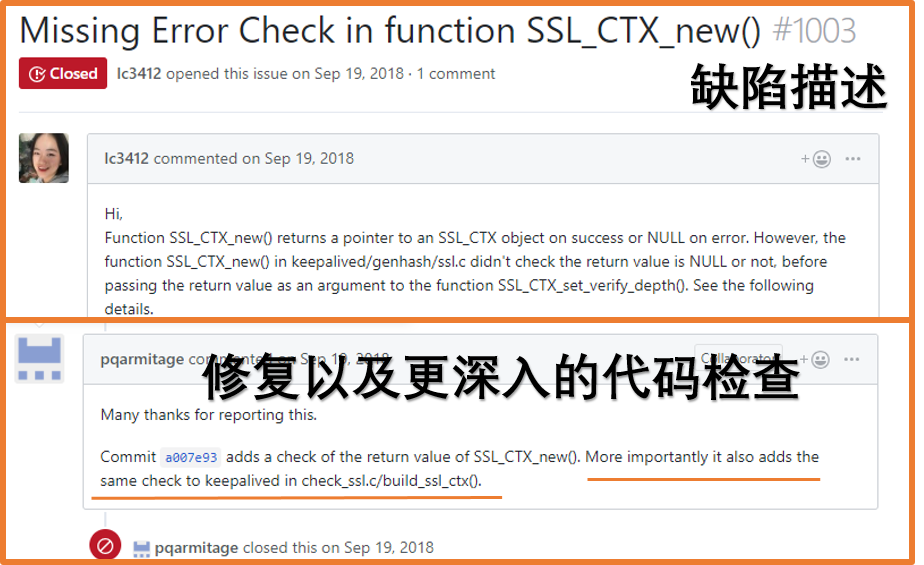
\includegraphics[width=0.8\linewidth]{figures/cp4-keepalived-fix.png}
	\caption{
		keepalived开发者根据本文缺陷报告进行深入的代码检查
	}
	\label{fig:4-4-keepalived-fix}
\end{figure}

\paragraph{开发者态度}
在缺陷报告的过程中,开发者展现出不同的态度。
一方面,开发者对缺陷报告进行积极响应,例如OpenSSL的开发者多数在1天就完成缺陷的修复。
另一方面,开发者则更希望作者提供实际的运行轨迹或者提供修复代码,而不仅仅是缺陷报告。
本文将与开发者的交流和讨论中总结出的特殊发现描述如下,
\begin{itemize}
	\item 开发者自身忽视接口使用的约束。
	在实际开发过程中,开发者难以做到完全正确。
	即使是简单的参数检查和返回值检查,在大量的代码中普遍存在这种缺陷。
	然而,这些缺陷难以通过人工的方式进行一一排查。
	特别地,当开发者认识到这些缺陷时,会对其他代码中同样的缺陷模式进行检测。
	如图\ref{fig:4-4-keepalived-fix}所示,在keepalived项目中,
	本文提交缺陷报告后,开发者不仅修复对应的缺陷,还对其他的代码进行类似缺陷的检测和修复。
	\item 特殊目的。
	虽然有些接口确实被误用,但是开发者故意为之或者在特殊的应用内无需修复。
	例如OpenSSL项目提供app/speed.c文件用于测试算法速度。
	因此在代码中,存在大量的缺少必要返回值检查的接口误用(IssueID-6575)。
	OpenSSL一个开发者认为这些误用在这个上下文中并不需要关注。
	然而,其他开发者认为这部分代码作为应用中的案例,是其他开发者的重要参考需要重视。
	开发者进行深入的讨论后,决定在后续的开发过程中进行统一处理(Assessed)。
	另一方面,由于C程序缺少异常处理机制,开发者会故意忽略部分异常检测,
	因为软件设计时本身就没有考虑这些情况。
\end{itemize}

总结来说,基于有效信息的缺陷报告能够获得开发者积极的反馈。
同时并不是所有的接口误用都会引起开发者的关注,
特别地有一些误用是开发者故意为之。
例如,提高运行效率、C程序无法支持的异常处理情况和接口本身的特殊性等等。


\section{本章小结}
\label{sec:4.5}
本章将C程序接口使用约束领域特定语言IMSpec和规模化接口误用缺陷检测方法IMChecker在实际项目中进行应用。
为帮助研究人员和开发者理解接口误用缺陷,本文整理C程序接口误用缺陷数据集APIMU4C。
该数据集包含来源于实际项目的接口误用案例库以及接口误用测试数据集,
从而帮助研究人员和开发者对检测工具的性能进行评估、针对性选择检测工具以及设计设计新的检测算法。
同时,本章设计并实现可视化支撑的C程序接口误用缺陷检测工具集Tsmart-IMChecker,
并将工具集应用于开源项目缺陷检测中。
应用结果显示,本文的方法能够有效地检测到实际项目中的未被发现的接口误用缺陷,并
在Linux内核、OpenSSL库和Ubuntu系统应用软件的最新稳定版本中提交75个实际缺陷报告。
其中62个已经被开发者确认,32个被开发者修复。